\documentclass[11pt,letterpaper]{article}
%% Coverpage Packs
\usepackage{wallpaper}

%%Query packs
\usepackage[utf8]{inputenc}
\usepackage{amsmath}
\usepackage{amsfonts}
\usepackage{amssymb}
\usepackage{url}
\usepackage{xcolor}
\usepackage{fullpage}
\usepackage{listings}
\usepackage{mathtools}
\usepackage{enumitem}
\usepackage{bm}
\usepackage{fixltx2e}
\usepackage{hyperref}
\usepackage{array}
\usepackage{multirow}
\usepackage{longtable}
\lstset{
	basicstyle=\ttfamily,
	columns=fullflexible,
	breaklines=true,
	postbreak=\mbox{\textcolor{red}{$\hookrightarrow$}\space},
}
\setlength\parindent{24pt}

%%Graphics packs
\usepackage{ulem}
\usepackage{geometry, tikz}
\usetikzlibrary{shapes,shadows,arrows.meta}
\geometry{
    a4paper,
    total={170mm,257mm},
    left=20mm,right=20mm,
    top=20mm,
}

%%Assumption/Constraint Packs
\usepackage{enumitem}

\title{Comp353 Warm-Up Report}
\author{Kai Nicoll-Griffith[40012407], Stephen Prizio[40001739], \\Giovanni Gebran[40018637], Nizar Belhassan[27519443]\\\\\bf{Team kzc353\_4}}

\begin{document}
	
	

	\begin{titlepage}
\tikz[remember picture,overlay] \node[opacity=1.0,inner sep=0pt] at (current page.center){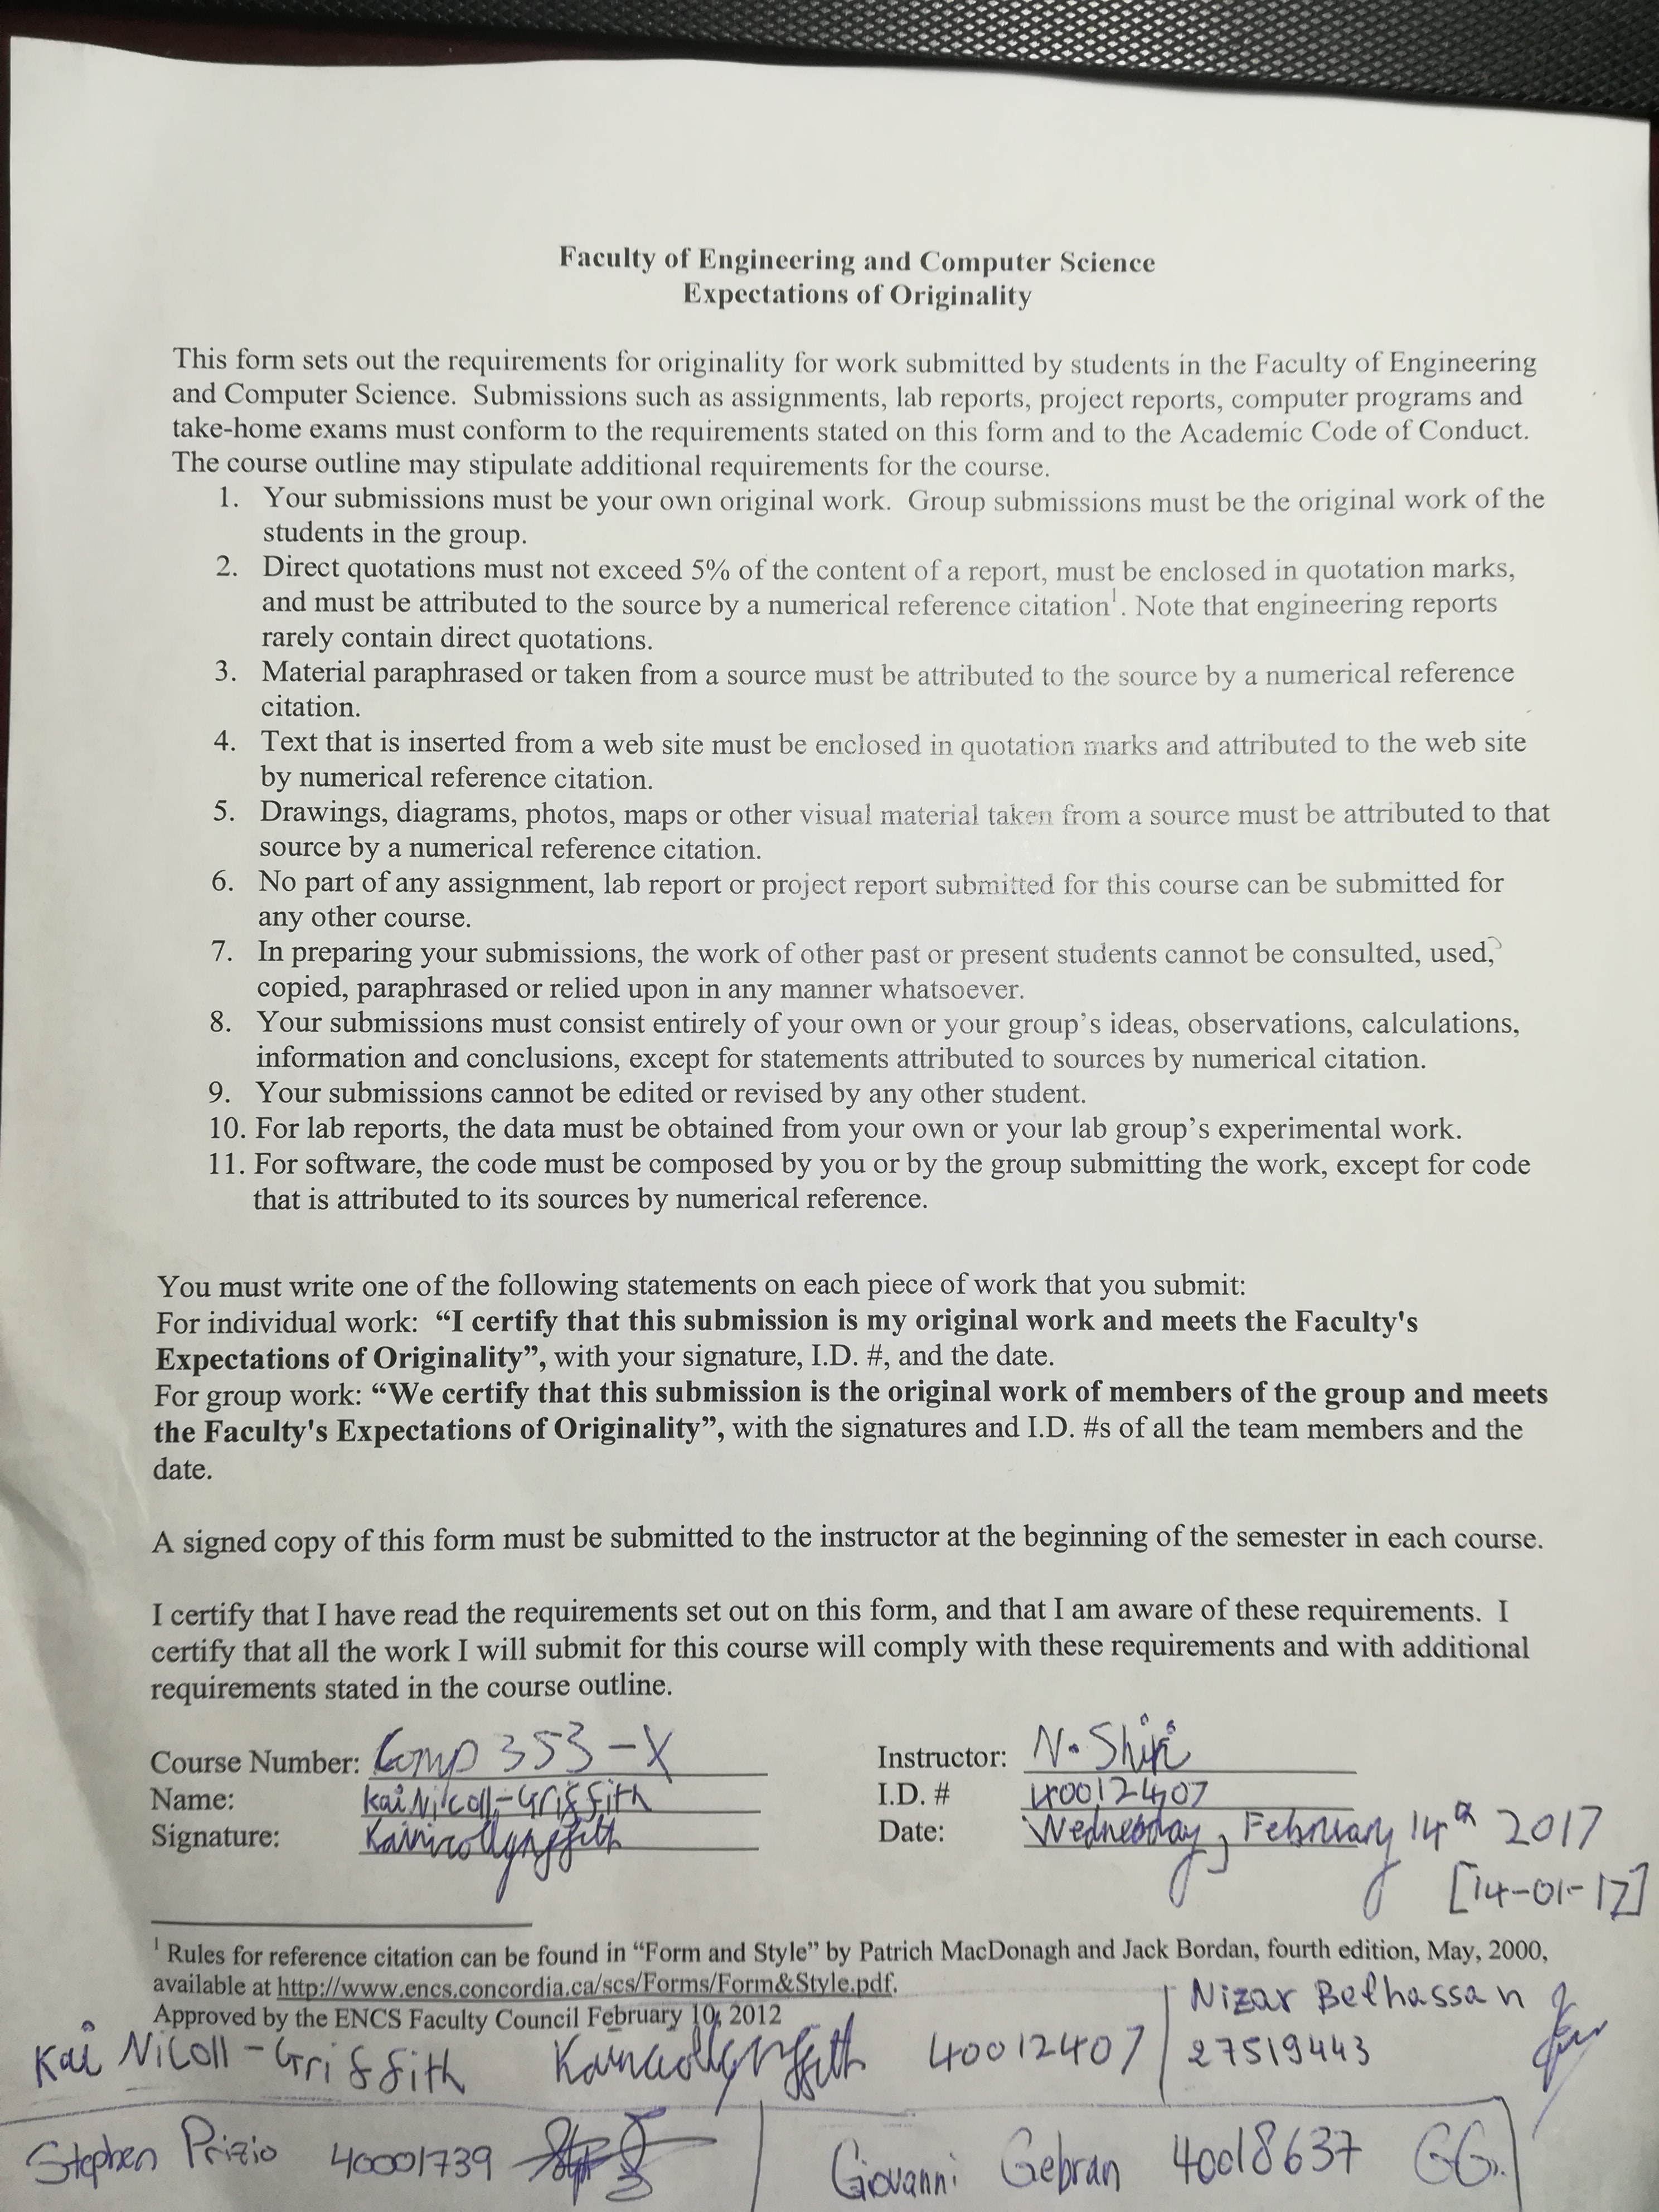
\includegraphics[width=\paperwidth,height=\paperheight]{originality.jpg}};
\end{titlepage}
	
		\maketitle
	
	
	\section{Assumptions}
	There are five relations:
\begin{enumerate}[label={\roman*.}]
	\item Students, 
	\item Teams,
	\item Members,
	\item Projects,
	\item Demos.
\end{enumerate}
	
	 Members is the many to one relationship between Students and Teams.
	The projects entity does not have any relation to the other entities.
	
	

	\section{Constraints}
	\begin{enumerate}[label={--}]
	\item Every student belongs to one and only team.
	\item Every team has at most 4 members.
	\item Every team has a unique demo.
	\item No student can do a demo without being a member of a team
	\item A project is a distinct entity independent of Students, Members, Teams, Demos.
	\end {enumerate}
	
	
	
		
	\pagebreak
	
	
		\newcommand{\XSHIFT}{7em}
	\newcommand{\YSHIFT}{0em}
	
	\tikzset{Item/.style={line width=0.14em}}
	\tikzset{Weak/.style={style=dashed}}
	\tikzset{EntitySet/.style={Item, rectangle,draw,fill={rgb:red,4;green,2;blue,1;white,9},inner sep=0.8em,drop shadow={shadow xshift=.5em,  shadow yshift=-.2em},node distance=14em}}
	\tikzset{WeakEntitySet/.style={EntitySet, Weak, Item}}
    \tikzset{Attribute/.style={Item,ellipse,draw,fill={rgb:red,1;green,1;blue,1;white,35},,drop shadow={shadow xshift=.35em, shadow yshift=-.1em},node distance=5.0em}}
    \tikzset{Relationship/.style={Item, diamond,draw,fill={rgb:red,0;blue,3;green,1;white,9},,drop shadow={shadow xshift=.25em,  shadow yshift=-.2em}, node distance=10em,aspect=3}}
	\tikzset{WeakRelationship/.style={Relationship, Weak, Item}}
    
    %%
    \tikzset{OneLine/.style={draw, =Stealth, line width=0.21em}}
 	\tikzset{AttributeLine/.style={draw, =Latex, line width=0.09em}}
    \tikzset{ManyLine/.style={draw={rgb:red,1;green,1;blue,1;black,10}, -{Stealth[fill={rgb:red,0;blue,0;green,1;black,6}, width=2em]},thick, line width=0.21em}}	
	
	\section{E/R Diagram and Schema}
	\subsection{Enitity Relationship Diagram}
	\begin{center}
		\begin{tikzpicture}
%Construct the entity->attribute relations
%%Students (SID, Name, gender, email), 
\node[EntitySet](students){\textbf{Students}};
\node[Attribute, above of=students](sid){\uline{SID}};
\node[Attribute, left of=sid](name){Name};
\node[Attribute, left of=sid,yshift=-3em,xshift=-3em](gender){Gender};
\node[Attribute, right of=sid](email){Email};

\path[AttributeLine](sid)--(students);
\path[AttributeLine](email)--(students);
\path[AttributeLine](name)--(students);
\path[AttributeLine](gender)--(students);

%%Members (SID, TID, dateJoined,role), 
\node[Relationship, below of=students, yshift=\YSHIFT](members){\textbf{Members}};
%\node[Attribute, right of=members](sid_mem){\uline{SID}};
%\node[Attribute, above of=members](tid){TID};
\node[Attribute, left of=members,below of=members,yshift=0.2em](datejoined){dateJoined};
\node[Attribute, above of=members,left of=members](role){Role};

%\path[AttributeLine](sid_mem)--(members);
%\path[AttributeLine](tid)--(members);
\path[AttributeLine](datejoined)--(members);
\path[AttributeLine](role)--(members);

%%Demos (SID, TID, Date, time, grade)
\node[EntitySet, right of=students, xshift=\XSHIFT](demos){\textbf{Demos}};
\node[Attribute, right of=demos](sid_dem){\uline{SID}};
\node[Attribute, below of=sid_dem](date){Date};
\node[Attribute, above of=demos](tid_dem){\uline{TID}};
\node[Attribute, right of=demos,above of=demos](time){Time};
\node[Attribute, left of=tid_dem](grade){Grade};

\path[AttributeLine](sid_dem)--(demos);
\path[AttributeLine](date)--(demos);
\path[AttributeLine](tid_dem)--(demos);
\path[AttributeLine](time)--(demos);
\path[AttributeLine](grade)--(demos);

%%Projects (PID, Name)
\node[EntitySet, below of=members,left of=demos, xshift=\XSHIFT, yshift=-3.5em](projects){\textbf{Projects}};
\node[Attribute,below of=projects](pid){\uline{PID}};
\node[Attribute, right of=projects,xshift=1em](name){Name};

\path[AttributeLine](pid)--(projects);
\path[AttributeLine](name)--(projects);

%%Teams (TID, LeaderID, NoOfMembers), 
\node[EntitySet, below of=members,yshift=\YSHIFT](teams){\textbf{Teams}};
\node[Attribute,left of=teams, xshift=-2.0em](tid){\uline{TID}};
\node[Attribute, below of=teams, yshift=-0.5em, xshift=1.5em](leaderid){LeaderID};
\node[Attribute, below of=teams, left of=teams, xshift=-2em, text width=4em](noofmem){NoOf Members};

\path[AttributeLine](tid)--(teams);
\path[AttributeLine](leaderid)--(teams);
\path[AttributeLine](noofmem)--(teams);

%Relation connections

\path[OneLine](students)--(members);
\path[ManyLine](members)--(teams);
\path[ManyLine](members)-|(demos);

		\end{tikzpicture}
	
	\end{center}
\subsection{Schemas}
	Students (\uline{SID}, Name, gender, email)\\
Projects (\uline{PID}, Name)\\
Teams (\uline{TID}, LeaderID, NoOfMembers)\\
Members (\uline{SID}, \uline{TID}, dateJoined, role)\\
Demos (\uline{SID}, \uline{TID}, Date, time, grade)\\
	\pagebreak
	
	\section{Queries}
	\paragraph{Queries} Below are the 9 queries implemented in SQL and their respective outputs.\\
	\\
	The database can be queried at the following url: \url{https://kzc353.encs.concordia.ca/index.php}.
	\begin{enumerate}
		
		\item Which student(s) is not a member of any team?
		\begin{verbatim}
		SELECT students.sid, students.name
		FROM students
		WHERE students.sid NOT IN (SELECT members.sid FROM members);
		\end{verbatim}
		Output:
		\begin{center}
			\begin{tabular}{ | c  c | c  c | }
				\hline
				sid & name & sid & name\\
				\hline
				40 & Helen-elizabeth Turn & 58 & Sabrina Woodley \\
				41 & Leila Bertot & 59 & Bridie Hansard \\
				43 & Sophronia Bruckner & 60 & Gertrudis Pykett \\
				44 & Eldin Roberds & 61 & Mord Tipperton \\
				46 & Alison Ivakin & 62 & Helen Hadkins \\
				47 & Izabel Dollin & 67 & Cecilia Ewbanck \\
				48 & Sallie Easlea & 68 & Faun Whales \\
				49 & Imogen Berrigan & 74 & King Cottrell \\
				53 & Stanford De Cleyne & 75 & Lorin De Vere \\
				55 & Etta Woolfenden & 76 & Lavina Wilks \\
				56 & Skippie Eglese & 77 & Arley Escoffer \\
				57 & Krissie Loges &  & \\
				\hline
			\end{tabular}
		\end{center}
		
		\item For each team, list its members
		\begin{verbatim}
		SELECT members.sid, students.name, members.tid 
		FROM members, students 
		WHERE students.sid = members.sid;
		\end{verbatim}
		Output:
		\begin{center}
			\begin{tabular}{ | c  c  c |  c c c | }
				\hline
				sid & name & tid & sid & name & tid \\
				\hline
				1 & Natal Gravett & 1 & 98 & Khalil Baudrev & 7 \\
				8 & Eal Bevar & 1 & 21 & Felita Martinson & 8 \\
				13 & Hadrian Finlaison & 1 & 69 & Shaun Bretland & 8 \\
				34 & Marcelline Wardlaw & 1 & 52 & Clerkclaude Vellacott & 9 \\
				
				66 & Camilla Ivanuschka & 2 & 87 & Hans Gilstoun & 9 \\
				85 & Ravner Edelston & 3 & 97 & Cirstofor Arnaldv & 9 \\
				90 & Daron Kenrat & 3 & 2 & Faustine Millsap & 10 \\
				100 & Laurie Emsden & 3 & 10 & Prue Primarolo & 10 \\
				
				84 & Tatum Rehorek & 4 & 15 & Maurv Pavinese & 10 \\
				20 & Job Klimsch & 5 & 16 & Roz Feavvour & 10 \\
				95 & Cobb Bernardeau & 5 & 3 & Evita Willbourne & 11 \\
				23 & Misha Dener & 6 & 11 & Lamar Sabbins & 11 \\
				
				89 & Gregor Paridge & 6 & 37 & Lavena Toe & 11 \\
				99 & Andrea Bramont & 6 & 51 & Michaelina Rosiello & 11 \\
				4 & Johnette Corkell & 7 & 22 & Kerstin Stairmon & 12 \\
				88 & Millard Skeleton & 7 & 82 & Phaedra Nyland & 12 \\
				\hline
				\hline
				5 & Patty Connett & 13 & 7 & Hastie Broggini & 19 \\
				9 & Orville Jarnell & 13 & 38 & Benito Jeste & 19 \\
				17 & Rafael Ever & 13 & 54 & Derron McGlynn & 19 \\
				19 & Diane-marie Kubasiewicz & 13 & 78 & Jase Langridge & 19 \\
				
				6 & Cozmo Storres & 14 & 27 & Marven Hedge & 20 \\
				12 & Eugene Killwick & 14 & 65 & Chelsey Kettle & 20 \\
				18 & Berti Yglesia & 14 & 28 & Templeton Rickaert & 21 \\
				45 & Ouintana Gidney & 14 & 32 & Karen Barens & 21 \\
				
				73 & Ruthe Coolson & 15 & 29 & Pammie Milch & 22 \\
				64 & La verne Officer & 16 & 86 & Ilario Hinrich & 22 \\
				83 & Codee Bevn & 16 & 30 & Darius Doreward & 23 \\
				96 & Orelie Boullin & 16 & 50 & Jeremiah O'Hern & 23 \\
				
				25 & Smith Pauwel & 17 & 31 & Petronia Shoveller & 24 \\
				72 & Milka Bridgnell & 17 & 70 & Nathanil Cockerham & 24 \\
				26 & Charlotta Josefsson & 18 & 33 & Colas Paff & 25 \\
				71 & Elinor Mottershead & 18 & 39 & Robinet Pethybridge & 25 \\
				\hline
				\hline
				81 & Konstance Bamburv & 26 & 80 & Leslev Stove & 28 \\
				93 & Maison Ciccetti & 26 & 92 & Ellene Potzold & 28 \\
				94 & Boony Innes & 26 & 42 & Jermaine Ridolfi & 29 \\
				14 & Bonny Brazenor & 27 & 79 & Gerrilee Jagson & 29 \\
				35 & Rodina Mebius & 27 & 91 & Kendricks Stainburn & 29 \\
				63 & Jackqueline Chant & 28 & 24 & Alberto Lathave & 30 \\
				& & & 36 & Jesse Baike & 30 \\
				\hline
			\end{tabular}
		\end{center}
		
		\item Who was not present in the demo of a team?
		
		\begin{verbatim}
		SELECT students.sid, students.name, members.tid
		FROM students, members
		WHERE students.sid = members.sid AND students.sid NOT IN (SELECT demos.sid FROM demos);
		\end{verbatim}
		Output:
		\begin{center}
			\begin{tabular}{ | c  c  c | }
				\hline
				sid & name & tid \\
				\hline
				12 & Eugene Killwick & 14 \\
				18 & Berti Yglesia & 14 \\
				25 & Smith Pauwel & 17 \\
				28 & Templeton & 21 \\
				37 & Lavena Toe & 11 \\
				54 & Derron McGlynn & 19 \\
				79 & Gerrilee Jagson & 29 \\
				89 & Gregor Paridge & 6 \\
				99 & Andrea Bramont & 6 \\
				\hline
			\end{tabular}
		\end{center}
		
		\item List the teams that have less than 4 members
		
		\begin{verbatim}
		SELECT teams.tid 
		FROM teams 
		WHERE teams.no_of_members < 4;
		\end{verbatim}
		Output:
		\begin{center}
			\begin{tabular}{ | c | c | }
				\hline
				tid & tid \\
				\hline
				2 & 18 \\
				3 & 20 \\
				4 & 21 \\
				5 & 22 \\
				6 & 23 \\
				7 & 24 \\
				8 & 25 \\
				9 & 26 \\
				12 & 27 \\
				15 & 28 \\
				16 & 29 \\
				17 & 39 \\
				\hline
			\end{tabular}
		\end{center}
		
		\item Given a TID, list the names of the members
		
		\begin{verbatim}
		SELECT students.name 
		FROM students, members 
		WHERE students.sid = members.sid AND members.tid = ??;
		\end{verbatim}
		For this query, the \textit{??} would be replaced with a TID. We expect values between 1 and 30, any other value would not return anything.\\
		\\
		Output for the query with a value of \textit{11} (i.e. TID = 11):
		\begin{center}
			\begin{tabular}{ | c | }
				\hline
				name \\
				\hline
				Evita Willbourne \\
				Lamar Sabbins \\
				Lavena Toe \\
				Michaelina Rosiello \\
				\hline
			\end{tabular}
		\end{center}
		
		\item Given a date, list all the teams that have demos on that day
		
		\begin{verbatim}
		SELECT DISTINCT demos.tid 
		FROM demos 
		WHERE demos.date = 'yyyy-mm-dd';
		\end{verbatim}
		For this query, the \textit{yyyy-mm-dd} would be replaced with a given date. Our schema uses the dates 2018-02-16 and 2018-02-17, any other values would not return anything. We also expect the parameter to be entered in this format. Any other format would result in an error.\\
		\\
		Output for the query with a value of \textit{2018-02-16}:
		\begin{center}
			\begin{tabular}{ | c | }
				\hline
				tid \\
				\hline
				1 \\
				10 \\
				11 \\
				7 \\
				5 \\
				8 \\
				12 \\
				6 \\
				18 \\
				20 \\
				22 \\
				21 \\
				9 \\
				17 \\
				3 \\
				\hline
			\end{tabular}
		\end{center}
		
		\item For each team that is not complete, list the TID and the capacity to increase
		
		\begin{verbatim}
		SELECT teams.tid, 4 - teams.no_of_members AS 'Capacity to Increase' 
		FROM teams 
		WHERE teams.no_of_members < 4;
		\end{verbatim}
		Output:
		\begin{center}
			\begin{tabular}{ | c | c | c | c | }
				\hline
				tid & Capacity to Increase & tid & Capacity to Increase\\
				\hline
				2 & 3 & 18 & 2 \\
				3 & 1 & 20 & 2 \\
				4 & 3 & 21 & 2 \\
				5 & 2 & 22 & 2 \\
				6 & 1 & 23 & 2 \\
				7 & 1 & 24 & 2 \\
				8 & 2 & 25 & 2 \\
				9 & 1 & 26 & 1 \\
				12 & 2 & 27 & 2 \\
				15 & 3 & 28 & 1 \\
				16 & 1 & 29 & 1 \\
				17 & 2 & 30 & 2 \\
				\hline
			\end{tabular}
		\end{center}
		
		\item Given a student Name or ID, find his/her team ID
		
		When given a student ID:
		\begin{verbatim}
		SELECT members.tid 
		FROM members 
		WHERE members.sid = ??;
		\end{verbatim}
		For this query, the \textit{??} would be replaced with the student's ID. We expect values between 1 and 100, any other value would not return anything.\\
		\\
		When given a student Name:
		\begin{verbatim}
		SELECT members.tid 
		FROM members, students 
		WHERE students.sid = members.sid AND students.name = 'Student name';
		\end{verbatim}
		For this query, \textit{Student name} would be replaced with the student's name.\\
		\\
		Output for the query with a value of \textit{1} or \textit{Natal Gravett}:
		\begin{center}
			\begin{tabular}{ | c | }
				\hline
				tid \\
				\hline
				1\\
				\hline
			\end{tabular}
		\end{center}
		
		\item Given a student Name or ID, find the names and SID of his/her teammates
		
		When given a student ID:
		\begin{verbatim}
		SELECT students.sid, students.name 
		FROM students, members 
		WHERE students.sid = members.sid 
		AND members.tid = (SELECT members.tid FROM members WHERE members.sid = ??) 
		AND students.sid <> ??;
		\end{verbatim}
		For this query, the \textit{??} would be replaced with the student's ID. We expect values between 1 and 100, any other value would not return anything.\\
		\\
		When given a student Name:
		\begin{verbatim}
		SELECT students.sid, students.name 
		FROM students, members 
		WHERE students.sid = members.sid 
		AND members.tid = 
		(SELECT members.tid 
		FROM students, members 
		WHERE students.sid = members.sid AND students.name = 'Student Name') 
		AND students.name <> 'Student Name';
		\end{verbatim}
		For this query, \textit{Student name} would be replaced with the student's name.\\
		\\
		Output for the query with a value of \textit{14} or \textit{Cozmo Storres}:
		\begin{center}
			\begin{tabular}{ | c | c | }
				\hline
				sid & name \\
				\hline
				12 & Eugene Killwick \\
				18 & Berti Yglesia \\
				45 & Ouintana Gidney \\
				\hline
			\end{tabular}
		\end{center}
		
	\end{enumerate}
	
\end{document}